\section{Photometry}

\begin{frame}{principal wide band photometric regimes}
\cite{mallama2017comprehensive}
\begin{itemize}
\item Johnson-Cousins system (Johnson et al. 1966, Cousins, 1976 and Cousins 1976)
\item Sloan system (Smith et al., 2002 and Fukugita et al., 1996)
\end{itemize}
\end{frame}



\section{Timing}

\begin{frame}{Moto della stella attorno al cm}
Se luce emessa dalla stella primari ha tempi caratteristici il moto ellittico dovuto alla presenza del pianeta produce variazioni nel cammino ottico della luce proporzionaleallo spostamento della primaria lungo la linea di vista
\begin{equation*}
    \tau_p=\frac{1}{c}\frac{a\sin{i}M_p}{M_*}
\end{equation*}
\end{frame}

\begin{frame}{Osservazioni di pulsar.}
Emettono segnale periodico regolare $\Pi\approx\si{\second}-\si{\milli\second}$. Il moto attorno al comune centro di massa Pulsar/pianeta causa una variazione del cammino ottico: il segnale arriva in anticipo o in ritardo.
Nel caso de lsistema Sole/Terra il sole percorre un'ellisse di semiasse maggiore circa $\frac{m_T}{\msun{}}a_T\approx\SI{500}{\kilo\meter}$: la differenza di cammino ottico causerebbe un $\Delta t\approx\SI{1}{\milli\second}$.
Sistemi non nati con la stella: formati in fase finale di evoluzione.
\end{frame}

\section{Microlensing gravitazionale.}

\begin{frame}{lente gravitazionale}
La presenza di materia (densit\'a di energia) distorce lo spazio-tempo e il la radiazione EM pu\'o essere deviata: la luce proveniente da un'oggetto lontano pu\'o essere deviata dal campo gravitazionale di un oggetto (lente) e quindi per l'oservatore risulta distorta e amplificata. 

\begin{definition}{Microlensing.}
Si parla di microlensing quando le immagini multiple dell'oggetto lontano non sono risolte.
\end{definition}
\end{frame}

\begin{frame}{Gravitational light bending}
\begin{figure}[!ht]
\centering
%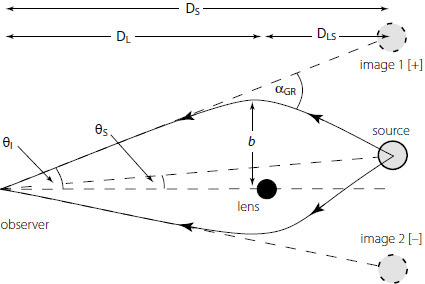
\includegraphics[width=(0.9\textwidth),height=\textheight,keepaspectratio]{lensing}
\caption{lensing.}
\end{figure}
\end{frame}

\begin{wordonframe}{Gravitational light bending}
\begin{definition}{Raggio di \sch{.}}
Il raggio di \sch{} \'e
\begin{equation*}
    R_S=\frac{2GM_L}{c^2}
\end{equation*}
\end{definition}
\begin{align*}
&\alpha_{GR}=\frac{4GM_L}{c^2b}=\frac{2R_S}{b}&\intertext{con la condizione che il parametro di impatto $b\gg R_S$}
\end{align*}
Lens equation:
\begin{equation*}
\theta_S=\theta_I-2R_S\frac{D_{LS}}{D_LD_S}\frac{1}{\theta_I}
\end{equation*}
\end{wordonframe}

\begin{frame}{Einstein radius.}
La sorgente lontana vedra la sua luminosit\'a amplificata dalla lente in proporzione all'Anello di Einstein
\begin{equation*}
    \theta_E^2=\frac{4GM_LD_{LS}}{c^2D_{OL}D_{OS}}
\end{equation*}
Le sorgenti galattiche possono essere stelle del nucleo galattico ($D_{OS}\approx\SI{10}{\kilo\parsec}$ e lenti tipic a met\'a strada).
Per $M_L\approx\msun{}$: $\theta_E\approx\si{\milli\arcsec}$.
Le dimensioni dell'anello di Einstein definiscono il livello di allineamento richiesto per avere una significativa amplificazione del segnale della sorgente.
Dimensioni lineari dell'anello di Einstein
\begin{align*}
    R_E=(1-y)\,d\theta=\sqrt{2y(1-y)R_Sd}
\end{align*}
con $d=D_{os}$, $yd=D_{LS}$, massime dimensioni lineari per $y=\frac{1}{2}$.
Il raggio di luce deve passare ad una distanza inferiore di $R_E$ dalla lente.
Inserendo quantit\'a tipiche per ricerca di esopianeti
\begin{align*}
&\theta_E\approx1.0(\frac{M_L}{\msun{}})\expy{\frac{1}{2}}(\frac{D_L}{\SI{8}{\kilo\parsec}})\expy{-\frac{1}{2}}(\frac{D_{LS}}{D_S})\expy{\frac{1}{2}}\si{\milli\arcsec}\\
&R_E\approx8.1(\frac{M_L}{\msun{}})\expy{\frac{1}{2}}(\frac{D_S}{\SI{8}{\kilo\parsec}})\expy{\frac{1}{2}}(\frac{D_LD_{LS}}{D_S^2})\expy{\frac{1}{2}}\si{\astronomicalunit}
\end{align*}
\end{frame}

\begin{frame}{Magnification}
\begin{figure}[!ht]
\centering
%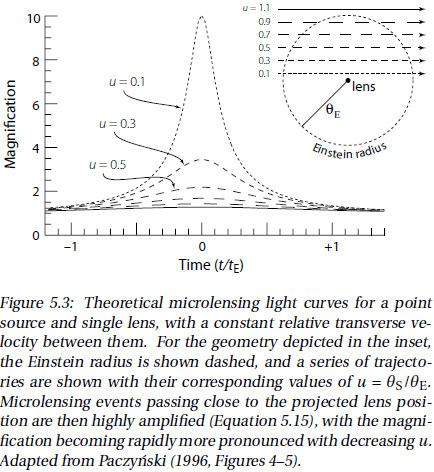
\includegraphics[width=(0.7\textwidth),height=\textheight,keepaspectratio]{lensinglcurves}
\caption{Microlensing magnification.}
\end{figure}
\end{frame}

\begin{frame}{Fatti}
\begin{itemize}
    \item In un cilindro di raggio $R_E$ e altezza $D_{OS}$ ho probabilit\'a $\frac{1}{100000}$ che ci sia una stella.
    \item Se la lente \'e costituita da pi\'u masse avremo una curva di luce con pi\'u picchi
    \item Nel caso di lente con sistema planetario la distribuzione dei picchi \'e detrminata dalla posizione dei pianeti: pi\'u efficace vicino all'anello di Einstein.
\end{itemize}
\begin{figure}[!ht]
\centering
%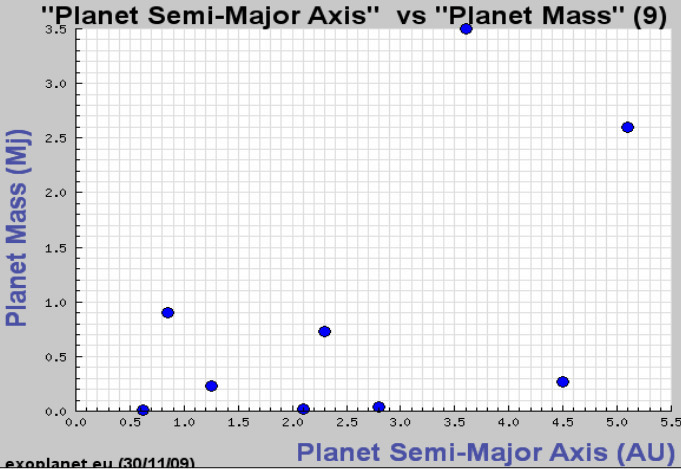
\includegraphics[width=(0.7\textwidth),height=\textheight,keepaspectratio]{mp-a-micro}
\caption{Massa pianeti vs semiasse per pianeti scoperti tramite microlensing.}
\end{figure}
\end{frame}

\section{Tecniche spettroscopiche (Misura velocit\'a radiale).}

\begin{frame}{Orbita stella attorno a CM}
\begin{figure}[!ht]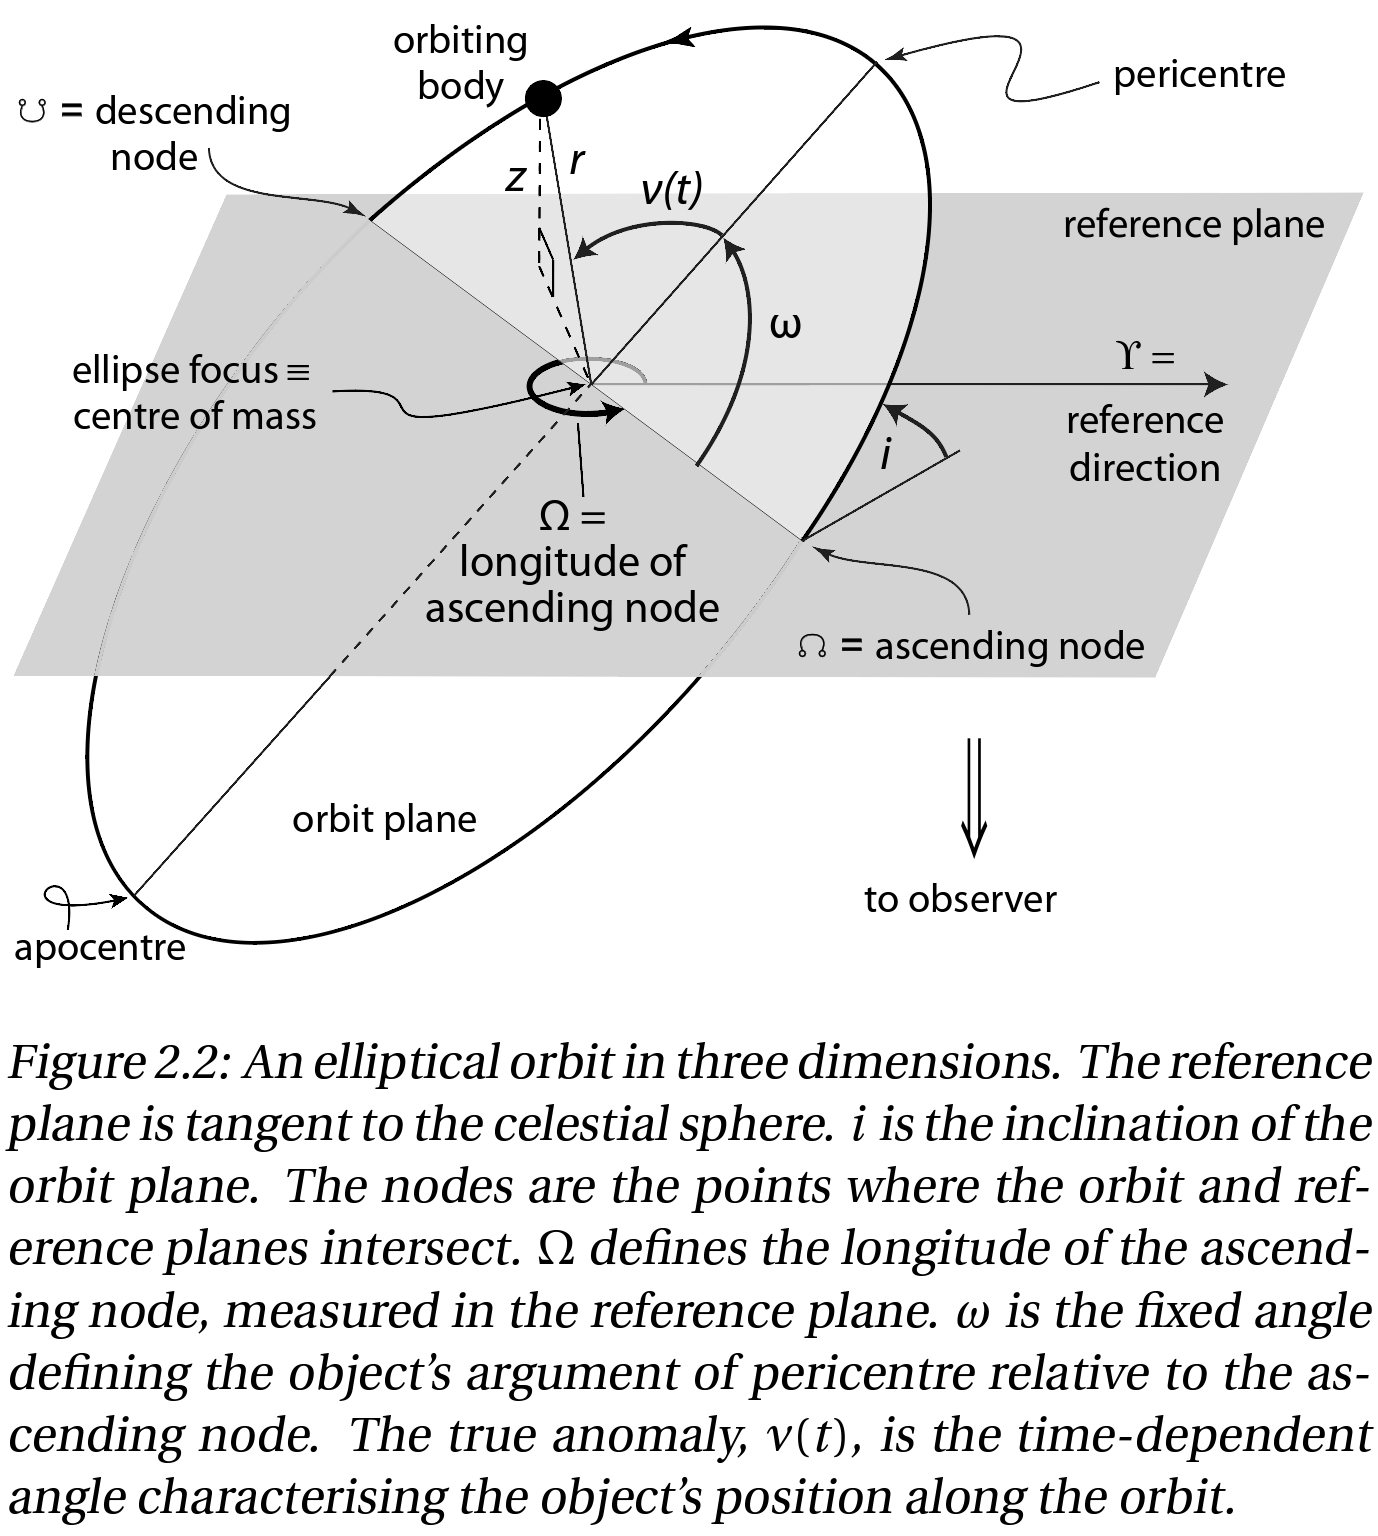
\includegraphics[trim={0cm 2cm 0 0},clip, keepaspectratio,height=0.5\textheight]{sightvelocity}\label{fig:sightvelocity}\end{figure}
\begin{align*}
&v_r=K[\cos{\omega+\nu}+e\cos{\omega}]\\
&K=\frac{2\pi}{P}\frac{a_*\sin{i}}{\sqrt{1-e^2}}\\
&K=\frac{2\pi}{P}\frac{a_*\sin{i}}{(1-e^2)\expy{1/2}}=(\frac{2\pi G}{P})\expy{1/3}\frac{M_p\sin{i}}{(M_p+M_*)\expy{2/3}}\frac{1}{(1-e^2)\expy{1/2}}
\end{align*}
\end{frame}

\begin{wordonframe}{Orbit specification}
\begin{columns}[T]\begin{column}{0.3\textwidth}
\begin{figure}[!ht]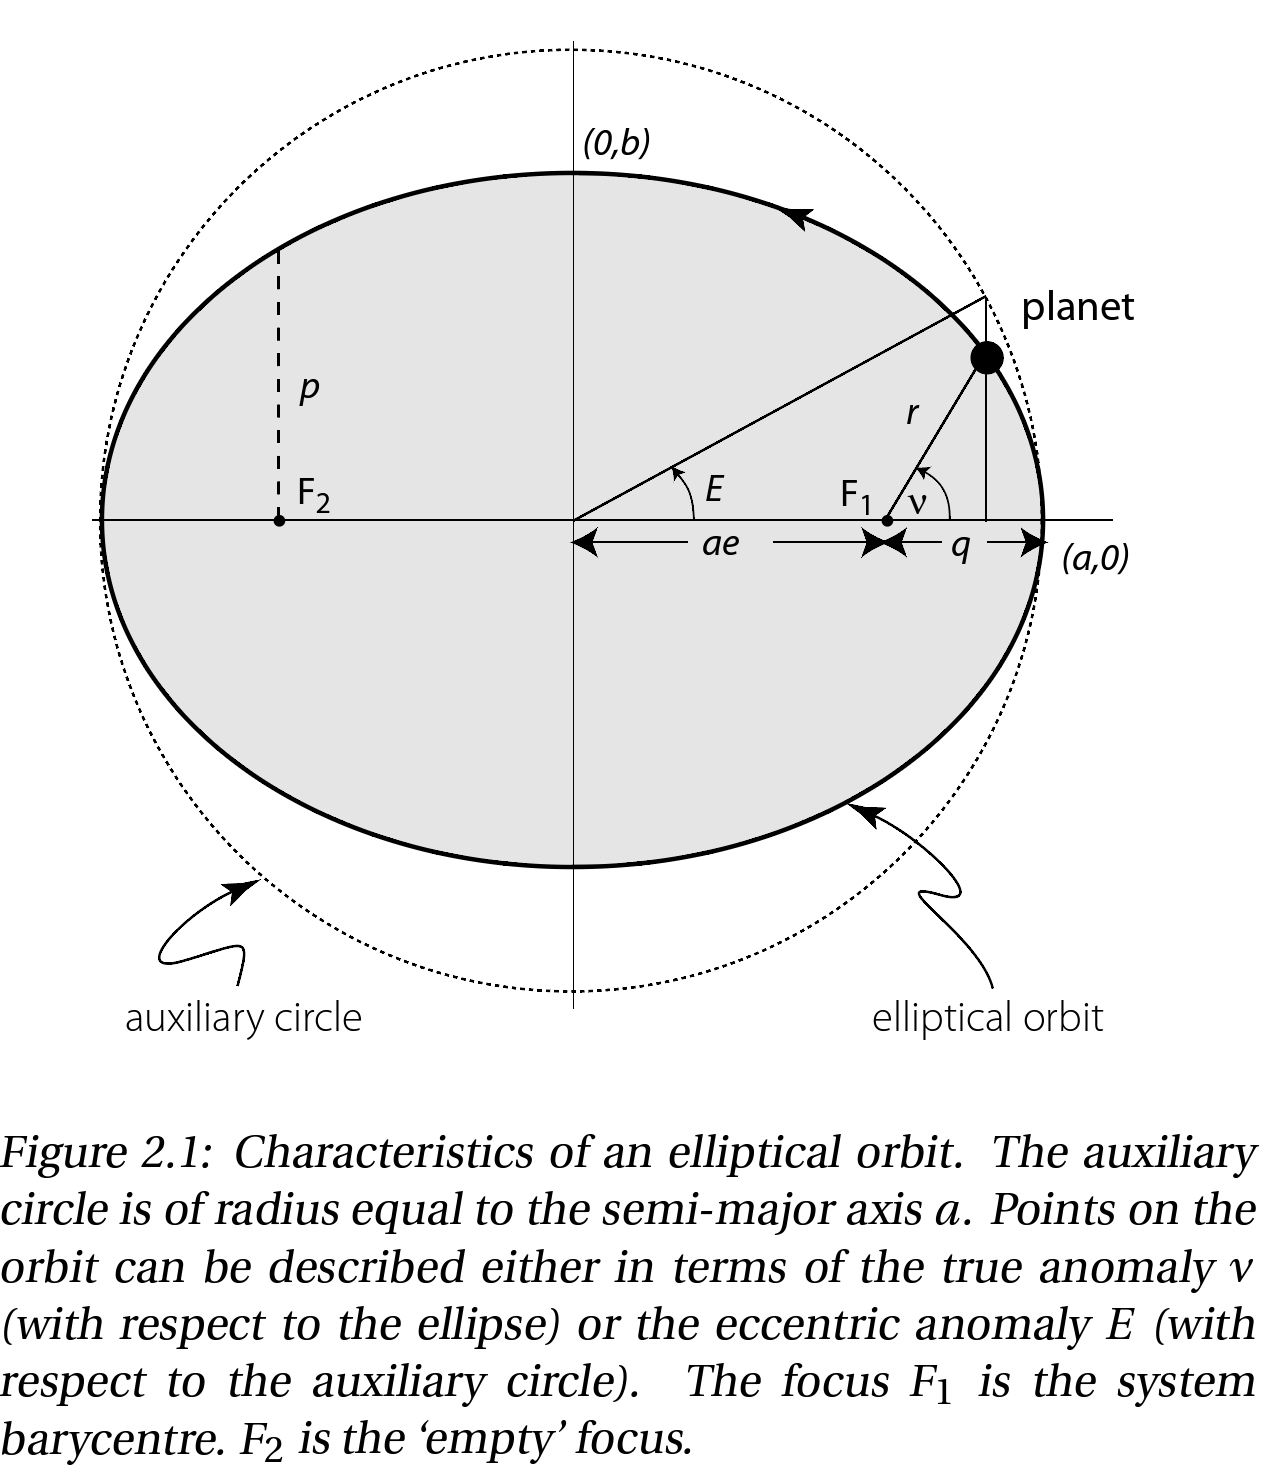
\includegraphics[trim={0cm 0cm 0 0},clip, keepaspectratio,width=0.99\textwidth]{ellipse}\label{fig:ellipse}\end{figure}
\end{column}\begin{column}{0.7\textwidth}
Ellipse: rel to focus $r=\frac{a(1-e^2)}{1+e\cos{\nu}}$, rel to center $\frac{x^2}{a^2}+\frac{y^2}{b^2}=1$.
\begin{align*}
&q=a(1-e)\\
&Q=a(1+e)\\
&p=a(1-e^2)
\end{align*}
$\nu(t)$ anomalia vera, $E(t)$ anomalia eccentrica, anomalia media $M(t)$, $t_p$ passaggio dal pericentro:
\begin{align*}
&\cos{\nu(t)}\frac{\cos{E(t)}-e}{1-e\cos{E(t)}}\\
&M(t)=\frac{2\pi}{P}(t-t_p)=n(t-t_p)
\end{align*}
\end{column}\end{columns}
\end{wordonframe}

\begin{wordonframe}{Variazione periodica velocit\'a radiale stella}
Variazione periodica della velocit\'a radiale dovuta al moto attorno al CM.
For the radial velocity semi-amplitude we have
\begin{align*}
&v_r=K[\cos{\omega+\nu}+e\cos{\omega}]\\
&K=\frac{2\pi}{T}\frac{A_*\sin{i}}{\sqrt{1-e^2}}\\
&K^2=\frac{G}{(1-e^2)}\frac{1}{a_*\sin{i}}\frac{M_p^3\sin^3{i}}{(M_*+M_p)^2}&\intertext{radial velocity measurement provide a value for mass function}\\
&\frac{M_p^3\sin^3{i}}{(M_*+M_p)^2}
\end{align*}
La terza legge di Keplero
\begin{equation}
(M^*+m_P)\sin^3{i}=\frac{4\pi^2a^3\sin^3{i}}{GP^2}
\end{equation}
$i$ \'e l'inclinazione dell'orbita rispetto al piano nella sfera celeste normale alla linea di vista.
\end{wordonframe}

\begin{frame}{Mass function}

Definisco la funzione delle masse
\begin{align*}
&f(M^*,m_P)=(M^*+m_P)\sin^3{i}\frac{m_P^3}{(M^*+m_P)^3}\\
&=\frac{4\pi^2}{GP^2}{a^*}^3\sin^3{i}\\
&f=\frac{PK_2^3}{2\pi G}&\intertext{$K_2$ is half the change in radial velocity.}\\
&f=\frac{M_1\sin^3{i}}{(1+q)^2}&\intertext{q \'e il rapporto tra le masse $M^*$ fratto massa oggetto non visibile $m_P$.}
\end{align*}
\end{frame}

\begin{wordonframe}{Radial velocity semi-amplitude}
Prendendo la coordinata z della stella lungo la linea di vista
\begin{align*}
&z=r(t)\sin{i}\sin{(\omega+\nu)}\\
&v_r=\dot{z}=K[\cos{(\omega+\nu)}+e\cos{\omega}]\\
&K=\frac{2\pi}{P}\frac{a_*\sin{i}}{(1-e^2)\expy{\frac{1}{2}}}
\end{align*}
Per il sistema Sole/Giove $K_k\approx\SI{12}{\meter\per\second}$ ($a=\SI{5.2}{\astronomicalunit}$, $P=\SI{11.9}{\year}$).
Sole/Terra $K_E\approx\SI{10}{\cm\per\second}$.
\end{wordonframe}

\begin{frame}{Keplerian observables}
\begin{columns}[T]\begin{column}{0.3\textwidth}
Descrizione orbita: $(a,e,P,t_p,i,\Omega,\omega)$.
\end{column} \begin{column}{0.7\textwidth}
\begin{figure}[!ht]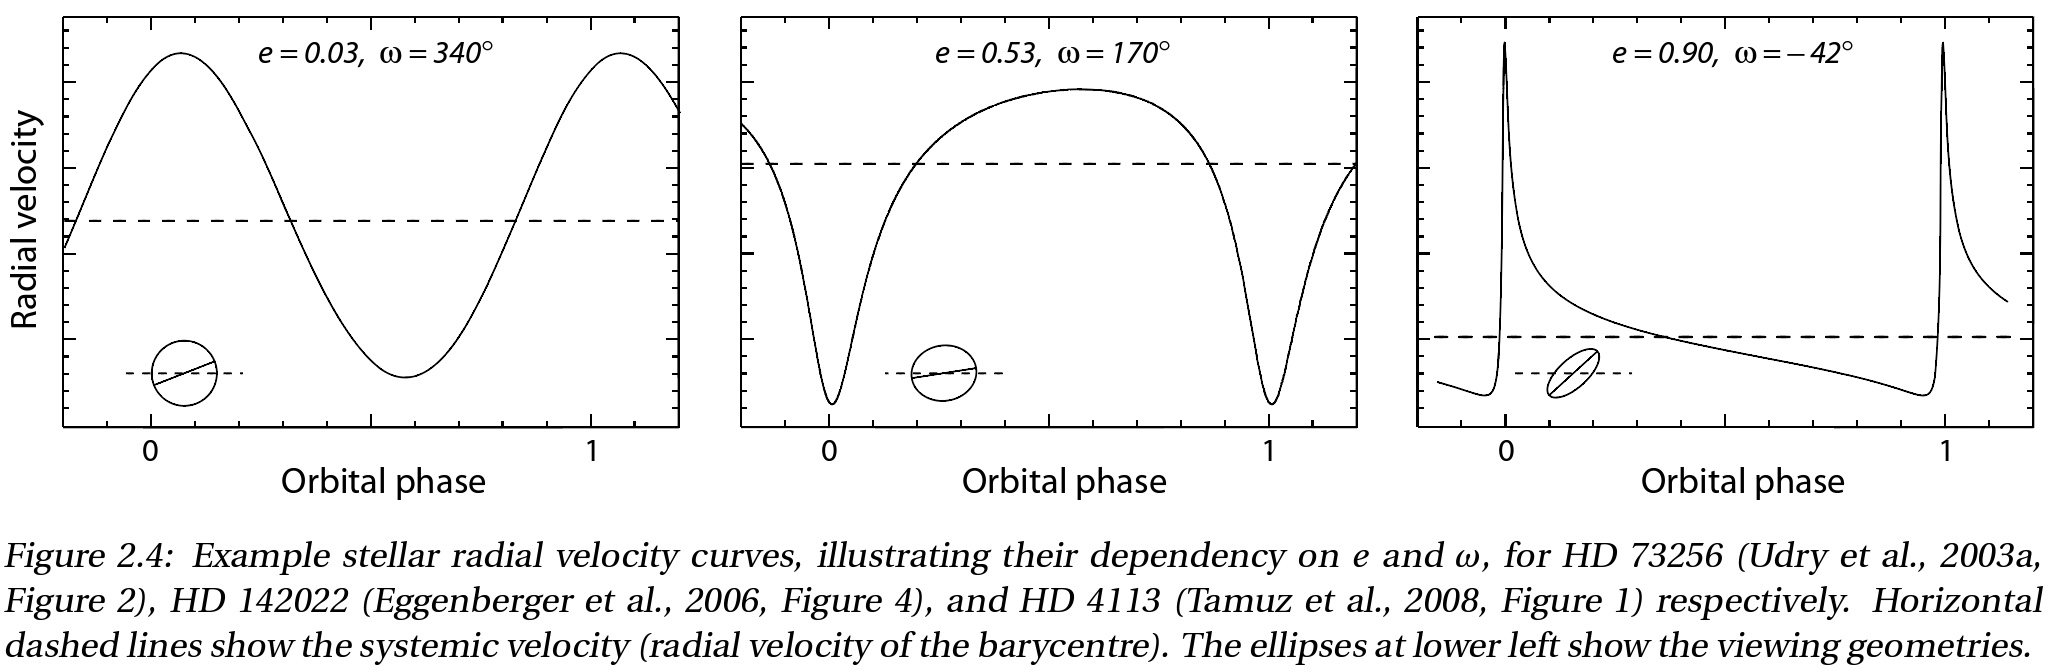
\includegraphics[trim={0cm 0cm 0 0},clip, keepaspectratio,width=0.9\textwidth]{orbitalphase}\label{fig:orbitalphase}\end{figure}
\end{column}\end{columns}
\begin{align*}
&v_r=K[\cos{(\omega+\nu(t))}+e\cos{\omega}]+\gamma+d(t-t_o)
\end{align*}
con $K(a,e,m\sin{i},P)$: ottengo e, P, $t_p$, $\omega$, $m\sin{i}$.
\end{frame}

\begin{frame}{Effetti di selezione}
\begin{columns}[c]\begin{column}{0.5\textwidth}
\begin{figure}[!ht]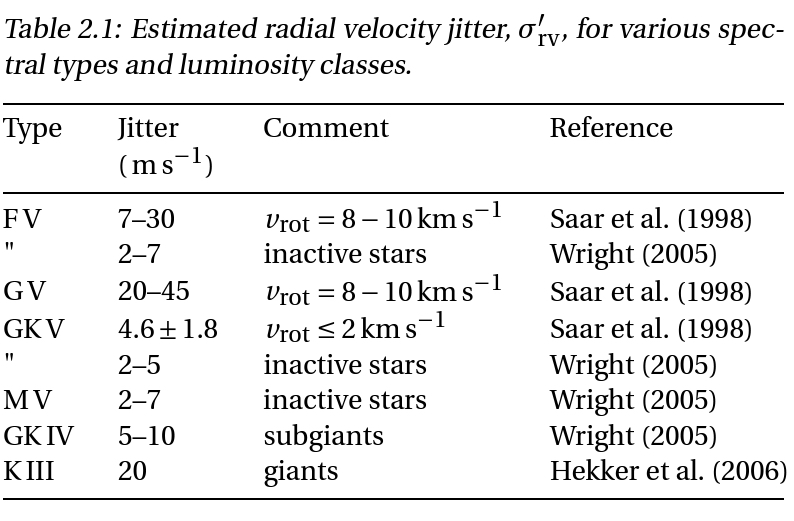
\includegraphics[trim={0cm 0cm 0 0},clip, keepaspectratio,height=0.49\textheight]{sigma-jitter}\label{fig:sigma-jitter}\end{figure}
\begin{figure}[!ht]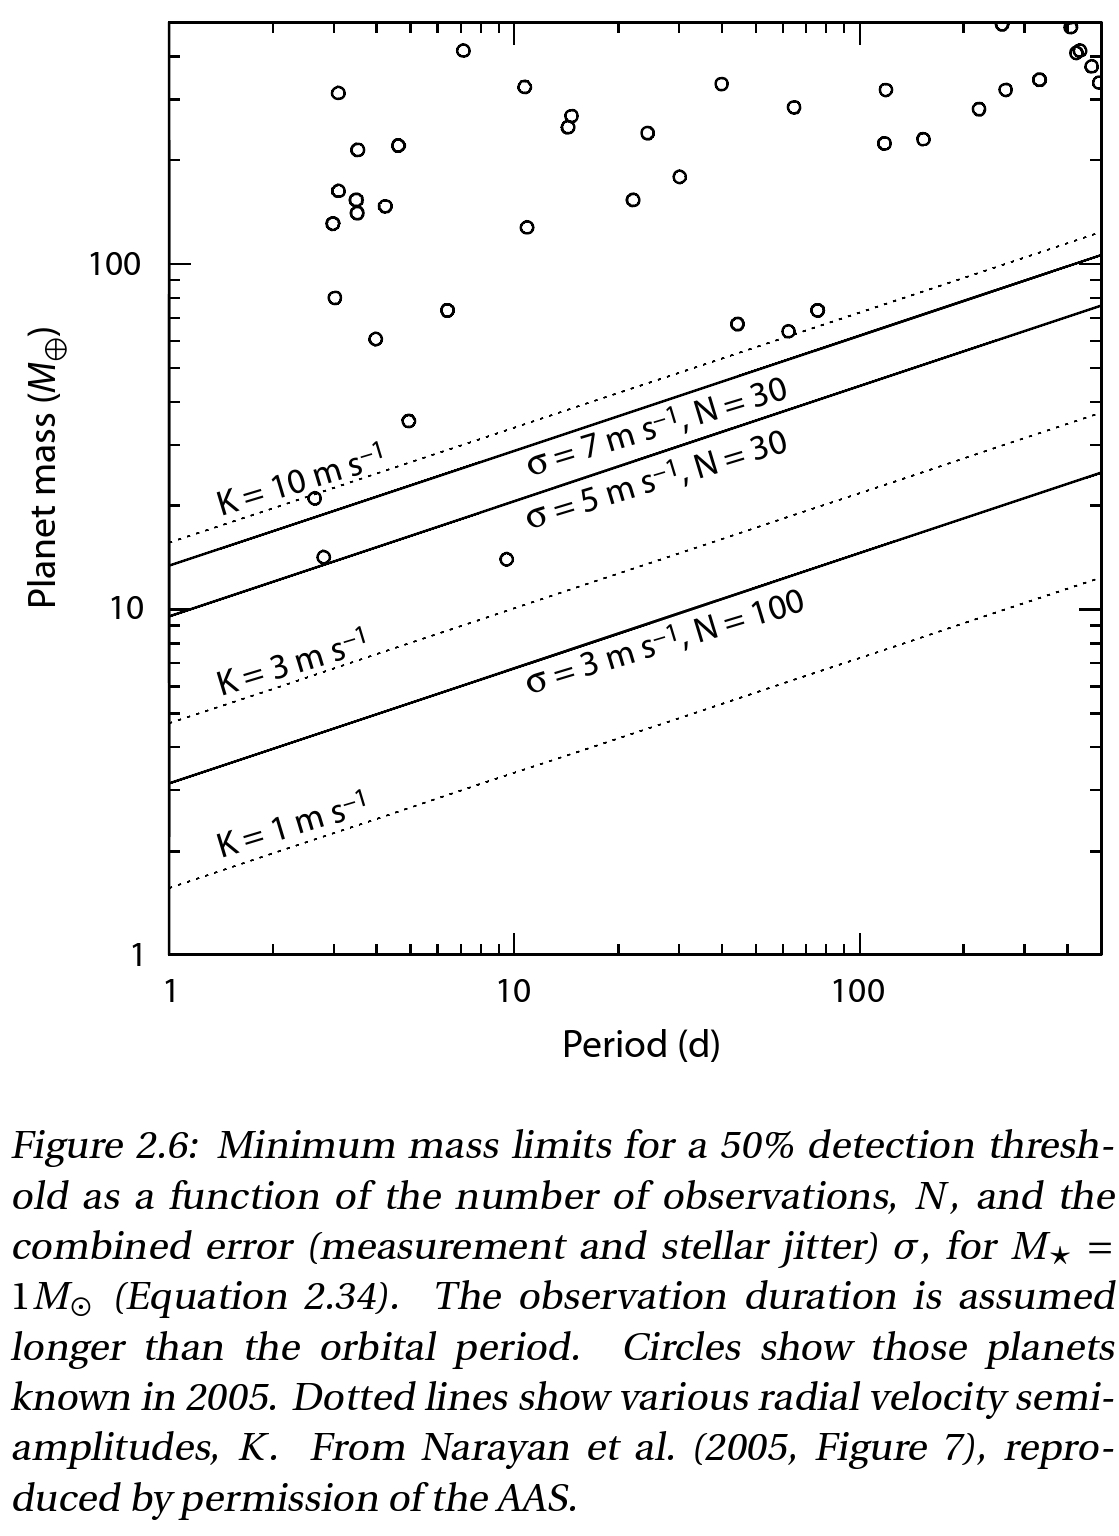
\includegraphics[trim={0cm 0cm 0 0},clip, keepaspectratio,width=0.49\textheight]{detection-th}\label{fig:detection-th}\end{figure}
\end{column}
\begin{column}{0.5\textwidth}
\begin{itemize}
\item SNR: Amplitude
\begin{align*}
K=\frac{\SI{28.4}{\meter\per\second}}{\sqrt{1-e^2}}\frac{M_p\sin{i}}{M_J}(\frac{P}{\si{\year}})\expy{-\frac{1}{3}}(\frac{M_*}{\msun{}})\expy{-\frac{2}{3}}
\end{align*}
Noise level: instrumental+stellar noise, number of measure: $s\propto N\expy{-1/2}$.
\item time span of observation.
\item shape of the orbit
\begin{align*}
&V(t)=V_z+K[\cos{(\nu(t)+\omega)}+e\cos{\omega}]\\
&\tan{(\frac{f(t)}{2})}=\sqrt{\frac{1+e}{1-e}}\tan{(\frac{E(t)}{2})}\\
&E(t)-e\sin{E(t)}=M(t),\ M(t)=\frac{2\pi}{P}(t-t_p)
\end{align*}

\end{itemize}
\end{column}
\end{columns}
\end{frame}


\section{Tecniche fotometriche: transiti.}

\begin{frame}{Observables of transit light curves}
\begin{columns}[c]\begin{column}{0.5\textwidth}
\begin{figure}[!ht]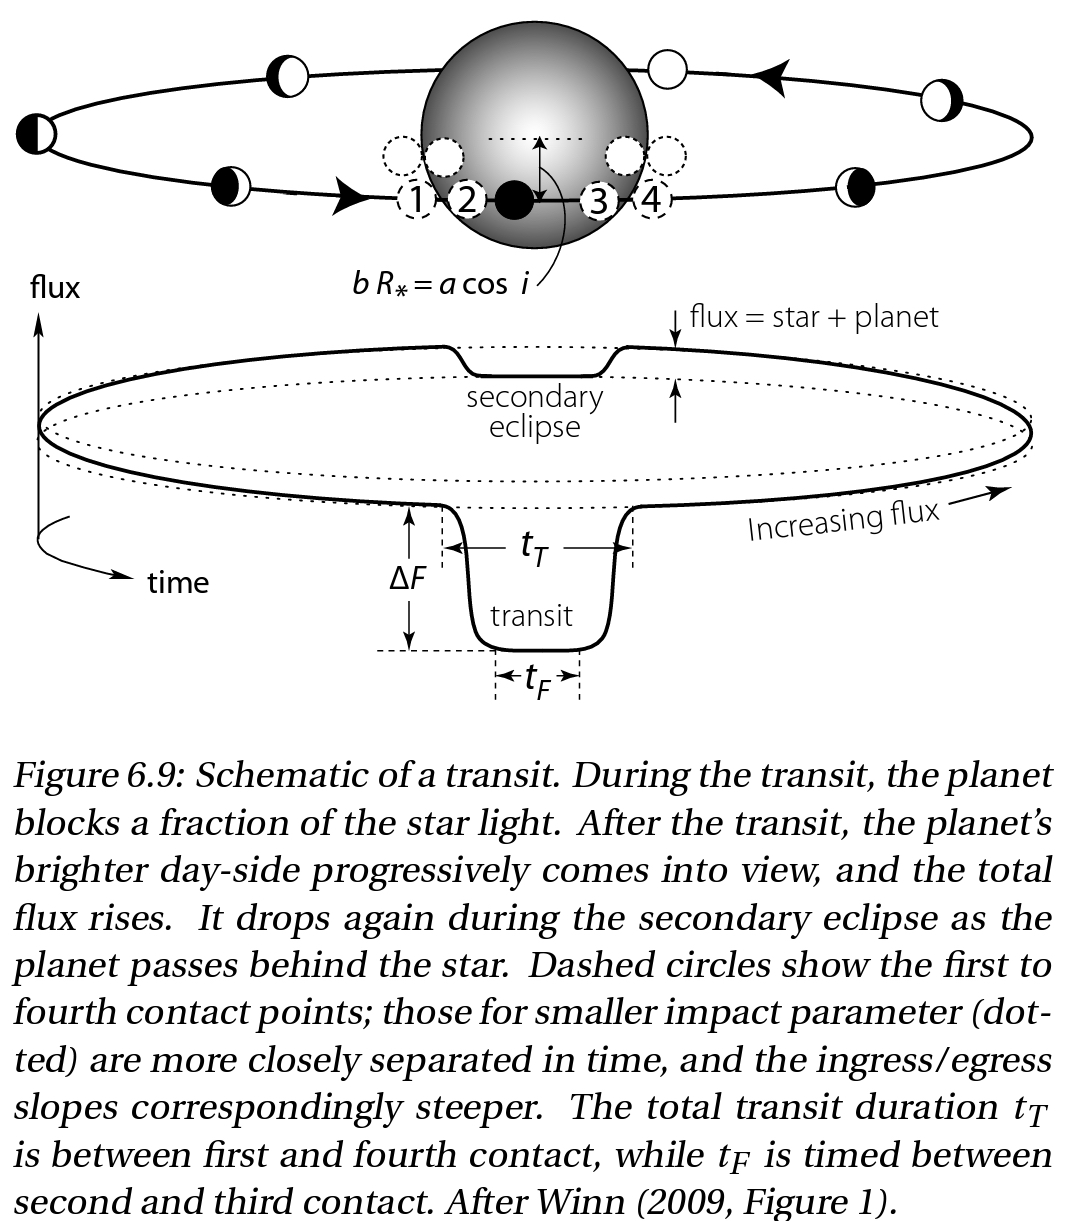
\includegraphics[trim={0cm 0cm 0 0},clip, keepaspectratio,height=0.45\textheight]{Tflux}\label{fig:Tflux}\end{figure}
\begin{figure}[!ht]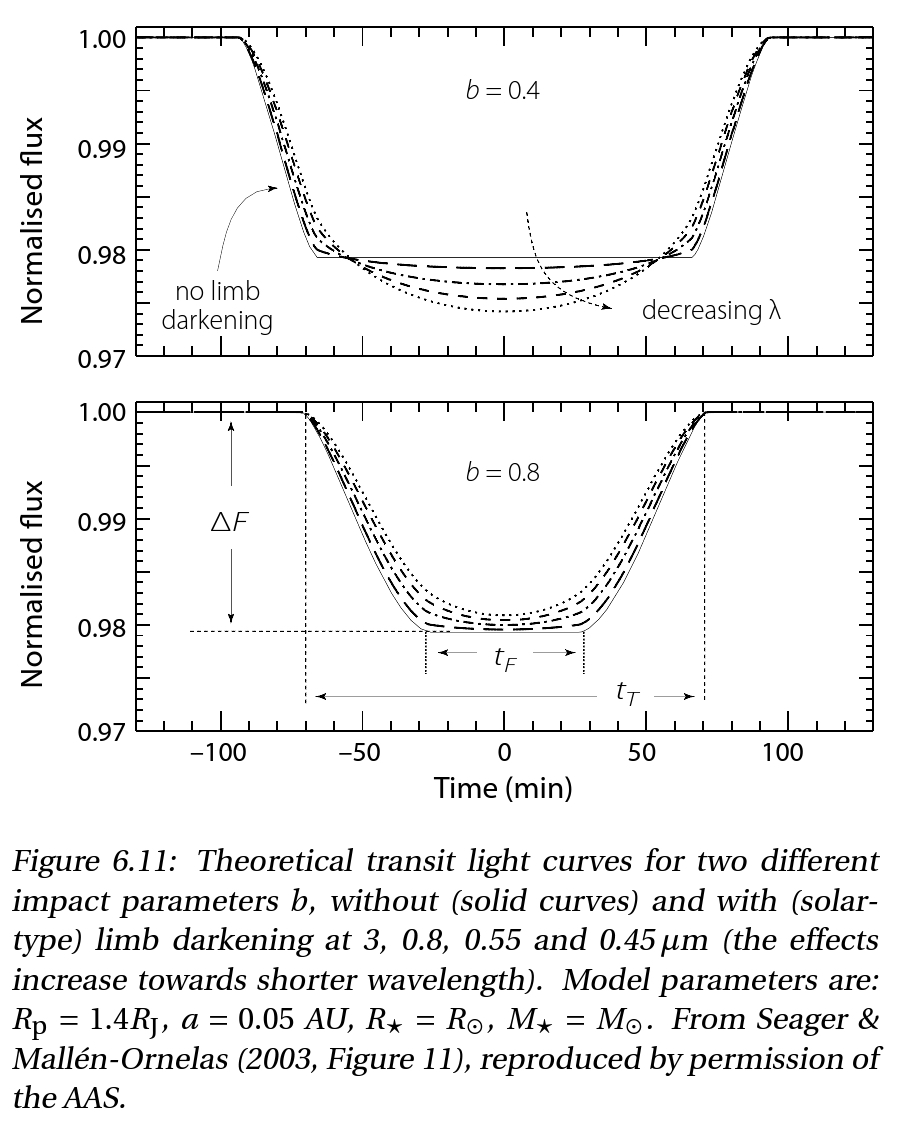
\includegraphics[trim={0cm 0cm 0 0},clip, keepaspectratio,height=0.45\textheight]{Tflux-b-lambda}\label{fig:Tflux-b-lambda}\end{figure}
\end{column} \begin{column}{0.5\textwidth}\end{column}  \end{columns}
\begin{itemize}
    \item Il periodo P.
    \item La profondit\'a del transito $\Delta F$.
    \item Intervallo di tempo tra 1-4 $t_T$.
    \item Intervallo di tempo tra 2-3 $t_F$.
\end{itemize}
\end{frame}

\begin{frame}{Transiti}

\begin{align*}
&\Delta F\approx(\frac{R_p}{R_*})^2\\
&t_T\approx13(\frac{M_*}{\msun{}})\expy{-\frac{1}{2}}(\frac{a}{\si{\astronomicalunit}})\expy{\frac{1}{2}}\frac{R_*}{\rsun{}}\si{\hour}
\end{align*}
La probabilit\'a che per un pianeta orientato arbitrariamente si possa osservare transito a eclisse secondaria \'e
\begin{equation*}
Pr\frac{R_*}{a}\approx0.005\frac{R_*}{\rsun{}}(\frac{a}{\si{\astronomicalunit}})\expy{-1}
\end{equation*}
data dall'area spazzata dall'ombra del pianeta sulla sfera celeste.
\end{frame}

\begin{wordonframe}{Probabilit\'a osservazione transito}
\begin{figure}[!ht]
\centering
%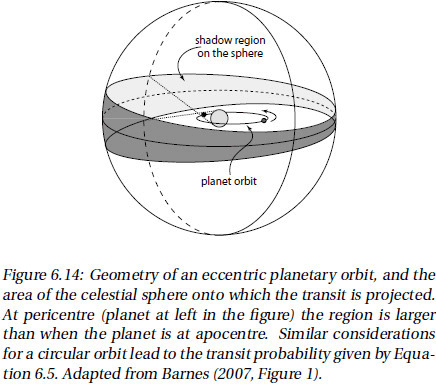
\includegraphics[width=(0.7\textwidth),height=\textheight,keepaspectratio]{sphereshadow}
\caption{Area della sfera celeste su cui \'e proiettato il transito.}
\end{figure}
\end{wordonframe}

\begin{wordonframe}{transito visto dalla terra}
\begin{figure}[!ht]
\centering
%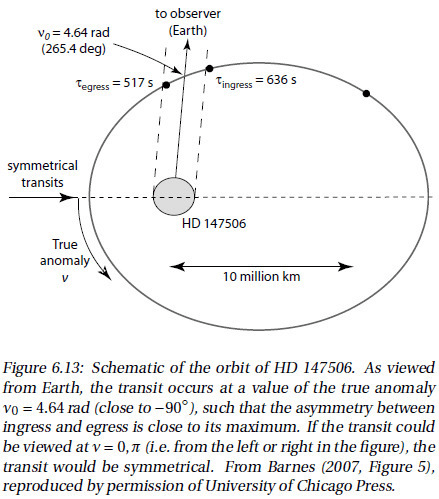
\includegraphics[width=(0.7\textwidth),height=\textheight,keepaspectratio]{transitex}
\caption{Transito visto dalla Terra.}
\end{figure}
\end{wordonframe}

\begin{wordonframe}{transiti: osservabili}
\begin{figure}[!ht]
\centering
%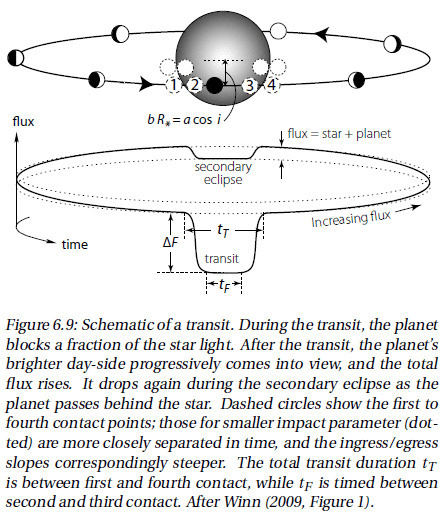
\includegraphics[width=(0.9\textwidth),height=\textheight,keepaspectratio]{transit}
\caption{Schematic of a transit and secondary eclipse (planet passes behind).}
\end{figure}
\end{wordonframe}

\begin{frame}{Fatti}
\begin{figure}[!ht]
\centering
%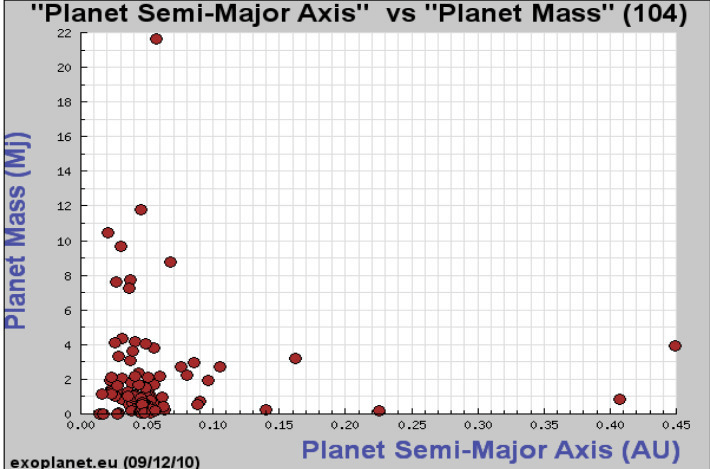
\includegraphics[height=0.9\textheight,keepaspectratio]{mp-atransit}
\caption{Massa pianeta vs semiasse per pianeti scoperti tramite transito.}
\end{figure}
\end{frame}

\begin{wordonframe}{Fatti}
\begin{itemize}
    \item Per un'eclissi totale Sole/Giove ho variazione $\Delta L\approx1\%$.
\end{itemize}
\end{wordonframe}